\chapter{Learning to find mountains}
\label{chapter4}
\thispagestyle{plain}

\section{Methods under evaluation}
Prominence, Isolation, Peak Clasification, Landserf Fuzzy Clasification, Unet,

\section{Input Data}
In Chapter \ref{chapter3} we saw how surface networks can be considered a useful representation of the topological properties of the shape that build the graphs are the Digital Elevation Models. The source we used for our files is the Shuttle Radar Topography Mission (SRTM) DEM provided by NASA \cite{Farr2007RGP}. SRTM DEM data are organized into a regular grid containing for each cell the elevation for the given coordinate, and they can be distinguished among STRM1 DEM and SRTM3 DEM. The distinction comes from the different resolutions they are subject to, i.e. how dense are the measurements available for a given area. DEM1 grids are relative to resolutions of 1 arc-second, while DEM3's resolution is in the order of 3 arc-seconds. Figure \ref{fig:dem_raster} showed an intuitive example how the elevation data can be organized in grids. 

For our work we focused mainly on the Switzerland territory and we used the SRTM1 DEMs with resolution of 1 arch-second, that in areas realtively far from the poles correspond approximately to 30m, i.e. we have a measurement of elevation every 30m. The data collected in SRTM1 DEM is then divided into a series of tiles of 3601x3601 cells for each tile and every one is spanning 1 degree in latitude and 1 degree in longitude. Tile N47E008, for example, contains the elevations arranged in the grid for the area between longitude from 8\degree E to 9\degree E and latitude from 47\degree N to 48\degree N.

\section{Algorithm for building the graph}
Among the methods illustrated in Chapter \ref{chapter3} for building surface networks from DEMs we opted for the algorithm of Shigeo Takahashi \cite{extracting_surface_topology}. However, we introduced some modifications to tackle a problem of misclassified critical points.
As Shigeo Takahashi said, classical methods like eight neighbours fail in extracting a number of critical points that respects the \textit{Euler-Poincarè formula}. The main problem in the eight-neighbours method is the appearance of many unwanted saddles due to lack of smoothness of DEMs, involving the invalidity for the formula. The proposed algorithm in \cite{extracting_surface_topology} tackles this problem by determining a unique surface interpolation from the given samples. For this purpose  \textit{triangulation} is used since it offers the most commonly adopted linear interpolation and does not incur unwanted critical points. A suggested triangulation in the paper is the \textit{Delaunay} because it avoids thin triangles that are undesirable for sound linear interpolations. Essentially, by introducing a triangulation the set of neighbours for each cell may reduce to a smaller number, avoiding the appearance of the unwanted passes. In fact, with triangulation we can define the neighbours of each sample and then introduce the criteria for critical points. If we consider a point P its neighbours are those points that are adjacent to P in the triangulation.
\begin{figure} 
\centering
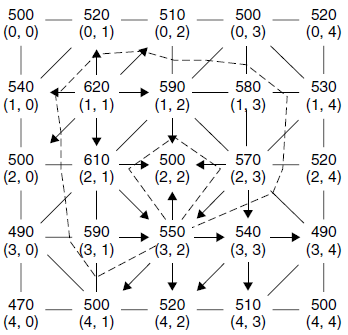
\includegraphics[width=8cm]{triangulation.png}
\caption{Triangulated DEM}
Figure illustrating how the neighborhood is established between the cells. Image courtesy Shigeo Takahashi \cite{extracting_surface_topology}.
\label{fig:triangulation}
\end{figure}
An example referred to the DEM raster in Figure \ref{fig:dem_raster} can be seen in Figure \ref{fig:triangulation}. 
\subsection{Criteria for finding Critical Points}
Shigeo Takahashi's algorithm considers a circular list of neighbours for each point P in a counter-clockwise (CCW) order with respect to xy-coordinates (or latitude/longitude if based on the DEM's coordinates). The criteria for critical points is as follows:

\textbf{peak} \quad \(|\Delta_+|\) = 0, \quad \(|\Delta_-|\) > 0, \quad \(N_c\) = 0

\textbf{pit} \qquad \(|\Delta_-|\) = 0, \quad \(|\Delta_+|\) > 0, \quad \(N_c\) = 0

\textbf{pass} \ \quad \(|\Delta_+|\) + \(|\Delta_-|\) > 0, \quad \qquad \(N_c\) = 4

where the following notation are used:

\textit{n} \ \ \quad the number of neighbors of \(P\)

\(\Delta_i\) \ \quad the height difference between \(P_i(i=1,2,...,n)\) and P

\(\Delta_+\) \quad the sum of all positive \(\Delta_i(i=1,2,...,n)\)

\(\Delta_-\) \quad the sum of all negative \(\Delta_i(i=1,2,...,n)\)

\(N_c\) \quad \ the number of sign changes in the sequence \(\Delta_1\), \(\Delta_2\),..., \(\Delta_n\), \(\Delta_1\)
\\
By using these criteria in combination with Delaunay triangulation it is possible to maintain the Euler-Poincarè formula. However, for our graph we decided to not use the triangulation, instead we kept all the eight neighbours and then applied the criteria. The reason for this choice is due to the fact that with triangulation more than 20\% of the saddles for the different areas we analyzed became local maxima. If our purpose would be a study of the semantics of these graphs the correctness of the topological rules would be fundamental. Instead, we are trying to understand if it is possible to categorize the nodes of the graph as being or not a mountain peak. Using the information about the category of the nodes in the features that carachterize them, i.e. knowing in advance what kind of critical point is a node (minimum, maximum or pass), increases the semantic knowledge we have about the graph. Instead, including many saddles in the set of local maxima would make the feature of the category for the nodes less important and less discriminative for the learning purpose. We decided, then, to build the graphs by using the above criteria for distinguishing among the different types of critical points but considering always the eight direct neighbours instead of making a selection based on triangulation. When considering a cell and its eight direct neighbours we may refer to them as \textit{patches}. An example of how triangulation would incorrectly assign a maximum to a patch that instead would not be a critical point can be seen in Figure \ref{fig:wrong_peak}. 

\begin{figure} 
\centering
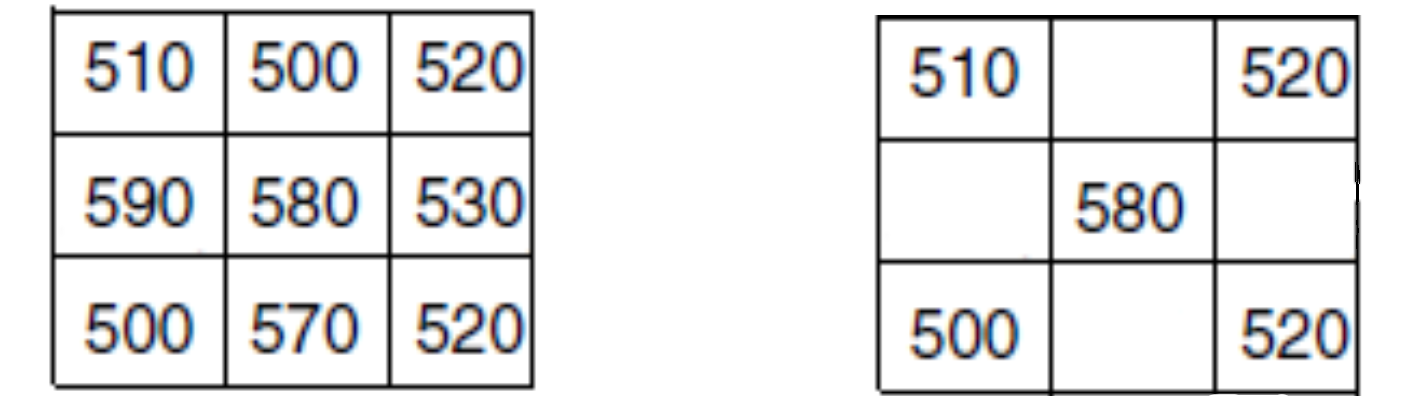
\includegraphics[width=8cm]{pictures/spurious_saddle.png}
\caption{Incorrect classification of cell with triangulation}
Figure illustrating how the cell with elevation 580, which is not belonging to any morphological class, would be added to the set of maxima in case of the illustrated type of triangulation.
\label{fig:wrong_peak}
\end{figure}

Finally, since we said that the data collected by STRM is organized in different tiles, particular attention should be given to the cells on the borders of the different grids. Indeed, each cell in the corner has only three neighbours, while each cell on the border (except the corner) has five neighbours. To tackle this problem we padded each tile's border with the cells from the adjacent tiles. For example, considering the grid of 3601x3601 cells for the tile N47E008, the cell at position (0,0) has as neighbours inside its tile the cells (0,1), (1,1) and (1,0). Then, to these internal neighbours are added the ones coming from the adjacent tiles, in this case the cell at position (3600,3600) from grid referring to N48E007, the cells (0,3600) and (1,3600) from N47E007 and the cells (3600,0) and (3600,1) from N48E008. Specular approaches are adopted for the other corners and borders of the tiles.


\subsection{Handling degenerate critical points}
There are two kinds of degenerate critical points that can arise when extracting them from DEMs: \textit{level regions} and \textit{duplicate passes}.

The level regions, or as we said in Chapter \ref{sec:mountain_peaks_from_dem} the planes, are those patches that all have the same altitude. These kind of regions can extend beyond the standard nine cells patch. They are the result of the discrete quantization that leads to limited precision of the height values. A simple solution may be to consider the entire group of points having the same elevation as a single point. However, as suggested by S. Takahashi, this may not be a good idea if the flat area is surrounding a critical point in its interior, like in Figure \ref{fig:flat_area}(a).
\begin{figure} 
\centering
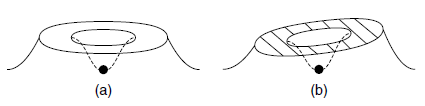
\includegraphics[width=8cm]{pictures/flat_area.png}
\caption{Level region}
A level region: (a) a level region surrounding a pit and (b) the effect of introducing a second ordering. Image courtesy S. Takahashi
\label{fig:flat_area}
\end{figure}
Instead, a second ordering is introduced, in the sense that when there is a tie between the elevations we consider a second factor for deciding which cell should be reviewed as higher. Similarly to the proposed method, in our implementation we used lexicographical ordering with respect to the xy-coordinates, where for x and y we can think at the row and column index inside the raster. Suppose, for example that cells (34,121) and (35,122) from the same grid have the same altitude 765m. In this case the second cell is considered as higher. Since the DEM is a set of samples on a single-valued function \(z = f(x,y)\), there are no two samples that have identical xy-coordinates. Indeed, if there is a tie for the x coordinate if the cells are on the same row of the grid, they cannot be on the same column, hence y would be different. Although this solution depend on the choice of x and y ordering, it enables uniform data manipulation by converting the degenerate critical points to non-degenerate ones. 

The second type of degenerate case are the duplicate passes from which is possible to extract two or more passes. With the criteria for the critical points we saw above each saddle is supposed to be connected to two maxima and to two minima points. Starting from the pass and following the two steepest ascents we would reach the two maxima while following the steepest descents we would reach the two minima. Degenerate saddles, instead, can be connected to three or four maxima and three or four minima respectively. In the case of three minima and maxima it means that there are six direct neighbours of the saddle whose path lead to a critical point; the three steepest descents lead to the minima, while the three steepest ascents lead to the maxima. The same consideration is valid for four minima and four maxima. Obviously, due to the arrangement of the raster as a matrix is not possible to have more than eight neighbours for a cell. The method of Shigeo Takahashi tackles this problem by splitting the degenerate saddles in two or three passes, depending on the number of changes in the sign. It modifies then also the criterion for the passes as:

\textbf{pass} \ \quad \(|\Delta_+|\) + \(|\Delta_-|\) > 0, \quad \qquad \(N_c\) = 2 + 2\(m (m=1,2,...)\)

 This problem, however, is not an issue because respecting the Euler-Poincarè formula is not our main concern. We kept then using saddles with more than four critical points connected.

\subsection{Connecting critical points}
We said that a surface network is a graph constituted by a set of vertexes, the critical points, and a set of edges, the critical lines, connecting the critical points. The ridges and channels constitute the physical path connecting the critical points. The ridges connect saddles to peaks (maxima) while the channels connect them to the pits (minima). The last type of morphological patch, the plane, is instead resolved by the second ordering factor and its never present in our graphs. Saddles are always connected to at least two maxima and two minima, with a maximum of four maxima and four minima. Instead there is never a connection between maxima and minima or between two saddles.

The graph is intended to be undirected, i.e. all the edges are bidirectional.  First, we find all the locations for the critical points by applying the criteria we described before. Considering a DEM we scan all the grid and consider always a cell and its eight neighbours and apply the crtieria to decide if it is a critical point and which type it is. Then, for finding the connections between the saddles and the minima and maxima we analyzed the adjacent cells to the ones in which we evaluated the presence of a saddle. Suppose \(P_0\) is one of these locations containing a saddle. Then, in the neighborhood of \(P_0\) there are other eight cells, \(P_1,P_2,...,P_8\). We ordered these cells such that they would constitute a circular sequence around \(P_0\); consider, as an example, the following clockwise ordered sequence based on the coordinates of the grid starting form the upper-left one \(\{P_1,P_2,P_3,P_4,P_5,P_6,P_7,P_8\}\). Then, in this sequence we look for the subsequences constituted by the higher neighbours and the ones constituted by the lower elevations.
Consider, as an example, \(P_0\)'s elevation as 700m, while the ones of the adjacent cells, in order from \(P_1\) to \(P_8\) as the sequence \(\{710,715,690,700,720,680,675,720\}\). Then among this sequence we can find the following subsequences of higher points: \(SH_1 = \{P_8,P_1,P_2\}\) with elevations \(\{720,710,715\}\) and \(SH_2 = \{P_4,P_5\}\) with elevations \(\{700,720\}\). The tie about considering \(P_4\) higher or lower than \(P_0\)  has been resolved with the second ordering. If the matrix coordinates start with (0,0) in the upper-left corner and we increase the values of the coordinates by moving down for the rows and moving right for the columns, then \(P_4\) results being a higher cell. The lower sequences are, instead, the following: \(SL_1 = \{P_3\}\) with elevations \(\{690\}\) and \(SL_2 = \{P_6,P_7\}\) with elevations \(\{680,675\}\).
An illustration can be seen in Figure \ref{fig:squences}.

\begin{figure} 
\centering
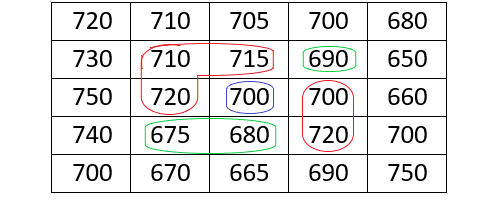
\includegraphics[width=10cm]{pictures/sequences.png}
\caption{Higher and lower subsequences}
Circled with blue we have the cell where the saddle is supposed to be located. Then around it there are four subsequences composed by the adjacent cells, two with higher elevations and are circled in red, two with lower elevations, circled in green.
\label{fig:squences}
\end{figure}

Among these subsequences we look for the highest value when dealing with higher sequences and for the lowest when dealing with lower sequences. These chosen cells will be the starting point for, respectively, steepest ascend path and steepest descend path. By applying this procedure in our example the subsequences reduce to \(SH_1 = \{P_8\}\), \(SH_2 = \{P_5\}\), \(SL_1 = \{P_3\}\) and \(SL_2 = \{P_6\}\). For finding the paths to the critical points we look for the steepest ascend path for the cells in the higher sequences and for the steepest descend path for the lower sequences. Consider, for example, the cell of \(P_8\) which constitute the starting point for the path to a maxima. For finding the steepest ascend we check the elevation of all its neighbours and choose as part of the path the one with the highest altitude. In this case would be the cell with 750 m. Then again we look at the adjacent cells to the last one added to the path and opt for the highest one. We continue applying this procedure and add cells to the path until we reach the location of a maxima found previously. For simplicity suppose that the cell is already the cell of a maxima. Similar procedure is applied for finding the connected minima. Figure \ref{fig:sequences_with_paths} illustrates how this procedure can find the paths to the four connected critical points.

\begin{figure} 
\centering
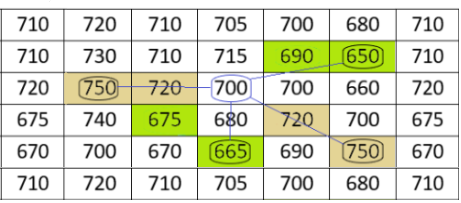
\includegraphics[width=11cm]{pictures/sequences_with_paths.png}
\caption{Paths and connections to the critical points}
This figure shows in brown the ridges, i.e. the paths from the saddle (circled in blue) to the maxima and in green the channles, i.e. the paths to the minima. The blue lines represent the edges in the graph. 
\label{fig:sequences_with_paths}
\end{figure}

Notice that the edges connecting the critical points don not follow strictly the paths. Indeed, surface networks graphs are an abstraction and the edges cannot follow the physical lines; edges are delimited by the coordinates of the saddle and the coordinates of the critical point. We can also see that the steepest ascend paths are part of the ridges, while the steepest descends are the channels. This procedure is highly inspired by the method of Shigeo Takahashi for splitting the saddles. 

\subsection{Degenerate paths}
Due to the lack of smoothness of the shape given by the DEM it may happen, as we can see in Figure \ref{fig:edge_rearrangement}, that both steepest ascend (descend) paths reach the same maxima (minima). In that case we removed the double edge and forced the connection with the closest maxima (minima) in terms of distance of cells inside the raster and which is not already present in the saddle edges. By making this reassignment of the duplicated edges we kept a slight recurrent structure inside the graph in the sense that we know for sure that all the saddles have four connected critical points, two maxima and two minima. The case with six or eight critical points can be easily reduced to four by splitting the saddle into two saddles with coincident location but different paths for different critical points. Keeping this small recurrence in the graph revealed to be useful when dealing with Deep Learning methods for graphs that require to have a common structure among the nodes. However, except of the saddles, the peaks and the pits have a really unpredictable number of connections, starting from one edge to even more than a hundred for few of them.

\begin{figure} 
\centering
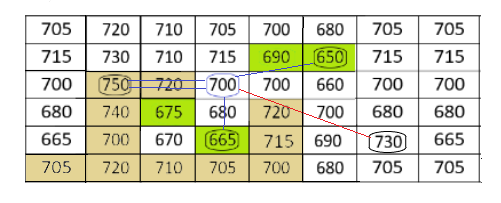
\includegraphics[width=13cm]{pictures/sequences_with_paths_degenerate.png}
\caption{Rearrangement of edges}
The blue lines represent the edges of the graph computed following the paths. The red line represents the new connection with a local maxima that was not reachable with the steepest ascent path. 
\label{fig:edge_rearrangement}
\end{figure}

\subsection{Enrichment of the graph with features}
The graph presented until now reflects a surface network (even though it is not respecting the Euler-Poincarè rule). It contains a set of vertexes, the critical points, and a set of edges, built over the critical lines. When dealing with Deep Learning for graphs some approaches require just the structure of the graph as input to learn from, but some other techniques can use some signals on the nodes or on the edges for better learning the properties of the nodes and the graph.

\subsubsection{Signals on the edges}
For methods that can handle weights on the edges, like \textit{node2vec} \cite{grover2016node2vec}, we used the slope as a representation of the steepness of the path. The signal of the slope, for each edge between nodes \textit{i} and \textit{j}, is then computed as:
\begin{equation} \label{slope}
s\textsubscript{ij} = \Delta \textsubscript{dist\textsubscript{ij}} / \mid\Delta \textsubscript{elev\textsubscript{ij}}\mid
\end{equation}

where \( \Delta \textsubscript{dist\textsubscript{ij}} \) is the distance expressed in meters between the cells where the two nodes of the graph are located, while \(\mid\Delta \textsubscript{elev\textsubscript{ij}}\mid\) is the difference of elevation between the two cells in absolute value. 

For the distance we had to consider that the Earth's surface is not flat and we cannot compute the distance like in an Euclidean plane. We used the \(haversine\) formula to calculate the great-circle distance between two points on a sphere given their longitudes and latitudes, i.e. the shortest distance over the Earth's surface (without considering any hill). First, we considered the location of the cells inside the grid relative to the tile's global position expressed as latitude and longitude, i.e. we calculated the specific latitude and longitude coordinate of each cell based on their position inside the grid. Then, the haversine formula is used to compute the distance as follows:
\begin{equation} \label{distance_haversine}
\Delta \textsubscript{dist\textsubscript{ij}} = R\cdot c 
\end{equation}

where \(R = 6,371m\) is the Earth's radius, while \(c\) is computed as:
\begin{equation}
c = 2\cdot atan2(\sqrt{a},\sqrt{(1-a)})
\end{equation}
with \(atan2(x,y)\) defined as the angle in the Euclidean plane, given in radians, between the positive x-axis and the ray to the point \((x,y)\neq(0,0)\). \(atan2(x,y)\) is intended to return a correct and unambiguous value for the angle \(\theta\) in converting from cartesian coordinates \((x,y)\) to polar coordinates \((r,\theta)\). It is defined as:
\begin{equation}
{atan2} (y,x)={\begin{cases}\arctan({\frac {y}{x}})&{\text{if }}x>0\\\arctan({\frac {y}{x}})+\pi &{\text{if  }}x<0\wedge y\geq 0\\\arctan({\frac {y}{x}})-\pi &{\text{if  }}x<0\wedge y<0\\+{\frac {\pi }{2}}&{\text{if }}x=0\wedge y>0\\-{\frac {\pi }{2}}&{\text{if  }}x=0\wedge y<0\\{\text{undefined}}&{\text{if  }}x=0\wedge y=0\end{cases}}
\end{equation}
Finally, \(a\) is the \textit{Haversine} computed as follows:
\begin{equation}
a = sin^2(\Delta \phi/2) + cos(\phi_i)\cdot cos(\phi_j ) \cdot sin^2(\Delta\lambda/2)
\end{equation}
where \(\phi_i\) is latitude for node \(i\), while \(\lambda_i\) is the longitude.

\subsubsection{Signals on the nodes}
Other methods for Deep Learning on graphs, like \textit{graphSAGE} \cite{graphSAGE}, during the learning process use a set of signals representing the properties of each node. Among the possible features of the nodes we considered both the topological properties of the graph, like the degree of the node or the type of critical point represented, and the terrain properties, like elevation or slope. In what follows consider that, although for the saddles we have a recurrent topology in the number of critical points to which they are connected, for the maxima and the minima it is not possible to replicate any structure, indeed they have a really large range of possible numbers of neighbours. Consider also that with \textit{graphSAGE} the edges represent just the existence of a relation between two nodes, i. e. that they are connected, and it is not possible to use signals on the edges. \textit{GraphSAGE} also requires that for each node we are using a vector of signals of fixed length, meaning that we are using the same features for each node. Then, for features like the slope which involve a relation between two nodes, if we would use all the signals that are possible to construct for that feature between the considered node and all of its neighbours we would have also really different sizes for the sets representing the signals. For being able to keep fixed the length of the vector containing the signals for the nodes, for features for which it is possible to calculate a variable number of signals depending on the number of neighbours we considered uniformly only the average, the maximum and the minimum of the set of signals for that feature. For example, for the slope, if a node has ten neighbours, first we computed all the ten possible slopes and we calculated the average, the maximum and the minimum values as the signals representing the node's slope. The features we identified for building the nodes' signals are then the following:
\begin{itemize}
\item \textit{elevation:} a real value expressed in meters representing the altitude of the cell inside the DEM where is located the node.
\item \textit{degree:} a natural number consisting in the number of neighbours to which the node is connected.
\item \textit{critical point type:} categorical attribute representing which kind of critical point there is at the location of the node. The possible values are \{peak,saddle,pit\}.
\item \textit{slope:} as we stated before the slope is computed based on the neighbours. We compute all the slopes with all the connected nodes by using the Formula \ref{slope} but without the absolute value when computing the difference of elevation:
\begin{equation} 
s\textsubscript{ij} = \Delta \textsubscript{dist\textsubscript{ij}} / \Delta \textsubscript{elev\textsubscript{ij}}
\end{equation} 
and then the following variants: 
\begin{itemize}
\item \textit{average slope:} the average value of the set of all the slopes
\item \textit{maximum slope:} the maximum slope in the set
\item \textit{minimum slope:} the minimum value in the set
\end{itemize}
\item \textit{absolute slope:} we compute all the slopes with all the connected nodes by using the Formula \ref{slope} and then its derived features:
\begin{itemize}
\item \textit{average absolute slope:} the average value of the set of all the slopes
\item \textit{maximum absolute slope:} the maximum slope in the set
\item \textit{minimum absolute slope:} the minimum value in the set
\end{itemize}
\item \textit{distance from neighbours:} this is another feature that depends on how many neighbours a node has. We compute all the distances by using the Formula \ref{distance_haversine} and then its derived features:
\begin{itemize}
\item \textit{maximum distance from neighbors:} the maximum distance in the set
\item \textit{minimum distance from neighbors:} the minimum distance in the set
\item \textit{average distance from neighbors:} the average value of the set of all the distances
\end{itemize}
\end{itemize}

\section{Ground Truth}
Deep Learning and in general Machine Learning models need trusted example data to learn from. Learning mountains from a graph can be achieved in different ways. In this work we tried mostly to learn which nodes of the graph correspond to the locations of the peaks of mountains. Note that here "peak of a mountain" is not the same of a "peak" of a surface network, even though they may coincide. Indeed in surface networks peaks are synonyms of maxima (always local, except of the case of global maxima that is the highest summit of the Earth, mount Everest). Instead, "peak of a mountain" or "summit of a mountain" are referred to the mountains that are registered in cartography or that traditionally recognized by society. This means that not all the maxima of the Earth's surface have been recognized as mountains. A local maxima that is almost flat or whose elevation is really low, for example a hill with really low slope, are often not registered neither in maps or public databases because society did not recognize them as mountains and didn't give a name to those locations. Also it is not even guaranteed that public databases and maps have the precise location for all the mountains. It depends often how historically they have been built and the social value that had those locations. Often these public data sets are mostly built by volunteers and cannot be assumed to be 100\% complete. Considering these aspects that influence where mountains are traditionally located we can state that not all the maxima are "real peaks", but it is not also really rare that the locations of the "real mountains" are tens of meters close to some node of the graph that corresponds to a maxima or, less often, coincident.

We said initially that we need trusted examples from which to learn. For our specific task we need then a set of "real peaks" or "trusted peaks" having a position that is known with acceptable certainty. These examples are said to constitute the \textit{Ground Truth}. They are not used only for training the machine learning models but also for making a comparison between which peaks the models we trained are able to extract and the ones extracted by other algorithms from literature. However, the reasons which makes impossible to have an exact overlap between the locations of the "real peaks" and the peaks of the surface network also makes impossible to have an ideal gold standard. Then we should account the fact that there is noise in the ground truth when we will evaluate the model output. It may happen for example that the model predicts as being a peak the node for a given location where it is not registered any "real summit", a so called false positive. However we may consider the fact that the peak was missing from the ground truth. Implementation of techniques for coping with label noise like \cite{FrenayV14} are not part of this work but it may be for future developments.

The data sets we used for our ground truth refer to the Switzerland territory. We used two different publicly available databases: OpenStreetMap\footnote{https://www.openstreetmap.org} (OSM) and SwissNames3D\footnote{https://shop.swisstopo.admin.ch/en/products/landscape/names3D}. We merged the peaks of the two databases by considering that their locations were overlapping when their distance was lower than 80m. We considered them potentially the same mountain summit and kept only one of the two after a manual inspection of the correctness of the choice. The resulting ground truth data set contains 12,788 peaks \cite{AI3D-DL-PE}. Their distribution can be seen in Figure \ref{fig:switzerland_peaks}.

\begin{figure} 
\centering
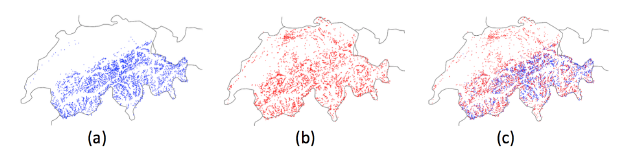
\includegraphics[width=13cm]{pictures/switzerland_peaks.png}
\caption{Mountain peaks distribution}
(a) contains the peaks from SwissNames3D, (b) peaks from OpenStreetMap and (c) their combination in the Switzerland territory. Image courtesy \cite{AI3D-DL-PE}
\label{fig:switzerland_peaks}
\end{figure}

\section{Label assignement to nodes}

\section{Graphs subsampling}

\section{Pre-processing of the input}
\section{Development of Graph learning-based methods}
\section{Dataset}
\section{Evaluation procedure}
%The  common output of all the methods is the geographic position of the mountain peak (latitude, longitude), which we also use to filter out all the extracted peaks that are out of the area under evaluation. To determine whether a candidate peak corresponds to a ground truth peak, we use a distance threshold (200m, in the evaluation described in Chapter \ref{eval}). The steps for the comparison, whose pseudocode is given in Algorithm \ref{algo:post-proc}, are as follows:
%\begin{itemize}
%\item Calculate the distance between each \textit{extracted peak} and every \textit{ground truth peak}.
%\item For each pair, save the tuple \textit{(extracted peak, ground truth peak, distance)}, only if the distance is lower than the established \textit{threshold}. 
%\item Order all tuples by increasing distance.
%\item Loop through the ordered list of tuples. Consider the extracted peak of the current tuple as a   \textit{True Positive} only if both the extracted and ground truth peaks have not already been used before to define other \textit{True positive} peaks; otherwise, discard the current tuple.
%\item The \textit{extracted peaks} that have a distance to all the ground truth peaks greater than the threshold are considered as \textit{False Positives}. Also, the extracted peaks that appear in a saved tuple, but have not been selected as true positive ones, because they were dominated by the  extracted peaks in some other tuple, are classified as \textit{False Positives}.
%\item The  \textit{ground truth peaks} for which no matching extracted peak has been identified are considered as \textit{False Negatives}.
%\end{itemize}

%\begin{algorithm}
%	\caption{Post-Processing}\label{algo:post-proc}
	%\begin{algorithmic}[1]
	%	\State $\textit{Distances} \gets \emptyset $
	%	\State $\textit{NGT} \gets \textit{length}(\textit{GTPeaks})$
	%	\State $\textit{NEPeaks} \gets \textit{length}(\textit{ExtractedPeaks})$
	%	\For{$i\gets 0 $ to $\textit{NGT} - 1$}
	%		\State $\textit{GTP} \gets \textit{GTPeaks}_i$
	%		\For{$j \gets 0 $ to $\textit{NEPeaks} - 1$}
	%			\State $\textit{EP} \gets \textit{ExtractedPeaks}_j$
	%			\State $\textit{Distance} \gets \textit{calculateDistance}(\textit{GTP},\textit{EP})$
	%			\If{$\textit{Distance} < 200$}
	%				\State $\textit{Distances}_{\textit{end}} \gets (\textit{EP},\textit{GTP},\textit{Distance})$
	%			\EndIf
	%		\EndFor
	%	\EndFor
	%	\State $\textit{TruePositives}  \gets \emptyset $
	%	\State $\textit{Distances} \gets \textit{sorted}(\textit{Distances})$
	%	\State $\textit{NDistances} \gets \textit{length}(\textit{Distances})$
	%	\For{$i\gets 0 $ to $\textit{NDistances} - 1$}
	%		\State $\textit{PeakTuple} \gets \textit{Distances}_i$
	%		\State $\textit{GTP} \gets \textit{PeakTuple}_{\textit{GTP}}$
	%		\State $\textit{EP} \gets \textit{PeakTuple}_{\textit{EP}}$
	%		\If{$\textit{GTP}$ in $ \textit{GTPeaks}$ and $\textit{EP}$ in $\textit{ExtractedPeaks}$}
	%			\State $\textit{TruePositives}_{\textit{end}} \gets \textit{PeakTuple}$
	%			\State $\textit{remove}(\textit{GTPeaks},\textit{GTP})$
	%			\State $\textit{remove}(\textit{ExtractedPeaks},\textit{EP})$
	%		\EndIf
	%	\EndFor
	%	\State $\textit{FalsePositives}  \gets \textit{ExtractedPeaks}$
	%	\State $\textit{FalseNegatives}  \gets \textit{GTPeaks}$
	%\end{algorithmic}
%\end{algorithm}

In summary:
\begin{itemize}
\item \textit{True Positives} are the extracted peaks that have a correspondence to a ground truth peak
\item \textit{False Positives} are the extracted peaks that  have no correspondence with a ground truth peak
\item \textit{False Negatives} are ground truth peaks that the method was not able to match to any extracted peak
\end{itemize}
\textit{True negatives}, i.e. locations that do correspond to non-peak sites, are more challenging to define because the number of potential candidates is overwhelmingly superior to those of the other types: the input DEM files are matrices of 3601x3601 pixels, of which only less than  1\%  are ground truth peaks.  To cope with such an unbalance, we  use the Precision-Recall curve in the assessment, rather than  other methods such as the ROC curve, as suggested in \cite{saito2015precision} for  scenarios with highly unbalanced classes.

%To better quantify the accuracy of the tested methods, we considered the mean distance error of each algorithm. In this way, the assessment considers not only the presence of a match between a ground truth  peak and an extracted peak, but also their distance (the lower, the better
